\paragraph{The gain is in the interval, at every horizon.} Fig.~\ref{fig:heat} shows the change of the RTT MAE and interval score of DS2S-E against S2S-E for every link and step. The interval score improves in every cell, most at short horizons on the satellite links. Almost all of the MAE gain comes from reporting the median instead of the mean. On the five links other than Starlink DL, the mean of DS2S-E changes the MAE by \MeanMAELo\% to $+$\MeanMAEHi\%, against \MedMAELo\% to \MedMAEHi\% for its median. Starlink DL is the one link where the mean also improves (\MeanMAESLDL\%), because its sawtooth is partly predictable.

\begin{figure}[t]
  \centering
  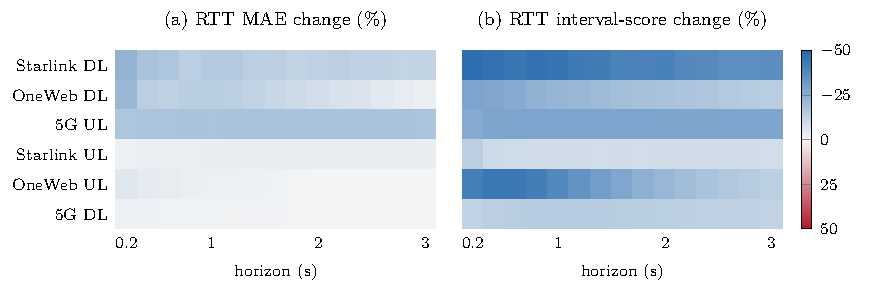
\includegraphics[width=0.85\linewidth]{figs_pdf/fr_heat.pdf}
  \caption{Change (\%) of the RTT MAE and of the calibrated 95\% interval score of DS2S-E against S2S-E per link and horizon step. Blue: DS2S-E is better.}
  \label{fig:heat}
\end{figure}

\paragraph{Conditional coverage.} Fig.~\ref{fig:condcov} breaks the coverage down by the volatility of the input window (deciles of the input RTT SD) and by horizon. The constant interval of S2S-E over-covers quiet windows and under-covers volatile ones. On Starlink DL it covers the calmest tenth at \CovConstSLDLdOne{} and the most volatile tenth at \CovConstSLDLdTen. Scaling the interval with the input SD reverses the error, because the future error grows much more slowly than the input SD. The largest decile deviation from 0.95 (coverage gap) of DS2S-E is \GapDSSLDL{} on Starlink DL, \GapDSQDL{} on 5G DL, and \GapDSQUL{} on 5G UL, against \GapConstSLDL{}, \GapConstQDL{}, and \GapConstQUL{} for the constant interval. The reduction is significant on these three links and on Starlink UL. On OneWeb it is not. DS2S-E widens its interval only \WidRatioOWDL{} times (DL) and \WidRatioOWUL{} times (UL) from the calmest to the most volatile tenth, while the error grows \ErrRatioOWDL{} and \ErrRatioOWUL{} times, and it covers that tenth only at \CovDSOWDLdTen{} and \CovDSOWULdTen. An SD-scaled interval with a tuned floor covers it at \CovNormTunedOWDLdTen{} and \CovNormTunedOWULdTen, so the input carries the warning and DS2S-E under-reacts to it.

\begin{figure}[t]
  \centering
  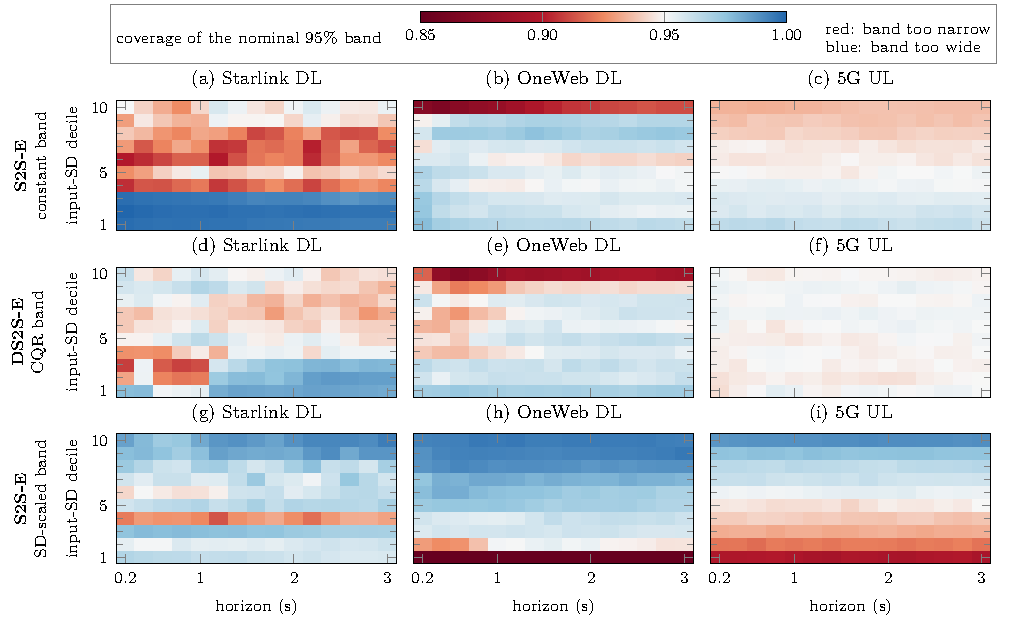
\includegraphics[width=\linewidth]{figs_pdf/fr_condcov.pdf}
  \caption{Conditional coverage of the calibrated 95\% RTT intervals on the test sessions per input-SD decile and horizon step. White: nominal 0.95. Blue: wider than needed. Red: too narrow (below 0.85 shares the darkest red). Bottom row: interval scaled by the input SD with a small floor.}
  \label{fig:condcov}
\end{figure}

\paragraph{Where the interval-score gain comes from.} We built intermediate intervals that change one ingredient at a time, all calibrated on the same sessions. Moving a constant interval from the S2S-E mean to the DS2S-E mean changes the score by \DecCentreLo\% to $+$\DecCentreHi\%, so the better center is not the source. Giving the S2S-E forecast the per-window width of DS2S-E, placed symmetrically, gains \DecWidthLoAbs\% to \DecWidthHiAbs\%. Placing it asymmetrically, as DS2S-E does, gains another \DecAsymLoAbs\% to \DecAsymHiAbs\%. The adaptive width carries most of the gain on Starlink DL and OneWeb UL, the skew on 5G UL.

\paragraph{How specific is the gain to the final model?} Table~\ref{tab:extent} lists every interval a deployed system could use. No interval around the S2S-E point forecast comes close to the quantile forecasters. The best of them is still \ExtBestPointLoAbs\% to \ExtBestPointHiAbs\% worse than DS2S-E on every link. The new inputs and decoder alone do not explain the gain either. S2S-AE-E shares them but outputs a mean, and it changes the interval score of S2S-E by only \ExtFrfullLo\% to $+$\ExtFrfullHi\%. \GaussSentence{} The linear quantile model LQR is within \ExtLQRMaxAbs\% of DS2S-E on every link and better on OneWeb UL and Starlink UL. DS2S-E is significantly better only on \LQRsigLinks, by \LQRsigLo\% to \LQRsigHi\%. The source of the gain is therefore the distributional output calibrated across sessions, which a linear model can exploit too. What the recurrent network adds is a better point forecast: against LQR it lowers the RMSE on all six links (\LQRRMSELoAbs\% to \LQRRMSEHiAbs\%, all significant).

\begin{table}[t]
\centering
\caption{Interval score (IS, ms) and coverage gap over input-SD deciles of the 95\% RTT intervals on the test sessions. SD-scaled: floor tuned on the calibration sessions. S2S-AE-E: inputs and decoder of DS2S-E with a scalar output. Bold: lowest IS of the link. GS2S-E \GaussSeedNote.}
\label{tab:extent}
\resizebox{\linewidth}{!}{%
\begin{tabular}{ll*{12}{r}}
\toprule
 & & \multicolumn{2}{c}{OneWeb DL} & \multicolumn{2}{c}{OneWeb UL} & \multicolumn{2}{c}{Starlink DL} & \multicolumn{2}{c}{Starlink UL} & \multicolumn{2}{c}{5G DL} & \multicolumn{2}{c}{5G UL} \\
\cmidrule(lr){3-4}\cmidrule(lr){5-6}\cmidrule(lr){7-8}\cmidrule(lr){9-10}\cmidrule(lr){11-12}\cmidrule(lr){13-14}
Forecast & Interval & IS & gap & IS & gap & IS & gap & IS & gap & IS & gap & IS & gap \\
\midrule
\tabinput{data/tab_extent.tex}
\bottomrule
\end{tabular}}
\end{table}
